\ylDisplay{Ruudustik} % Ülesande nimi
{Taavi Pungas} % Autor
{lõppvoor} % Voor
{2014} % Aasta
{G 1} % Ülesande nr.
{3} % Raskustase
{
% Teema: Elektriahelad
\ifStatement
Traadist on valmistatud 2x2 ruudustik (vt joonist), iga väikese ruudu külje takistus on $r=\SI{1}{\ohm}$. Leidke punktide A ja B vaheline takistus.

\begin{center}
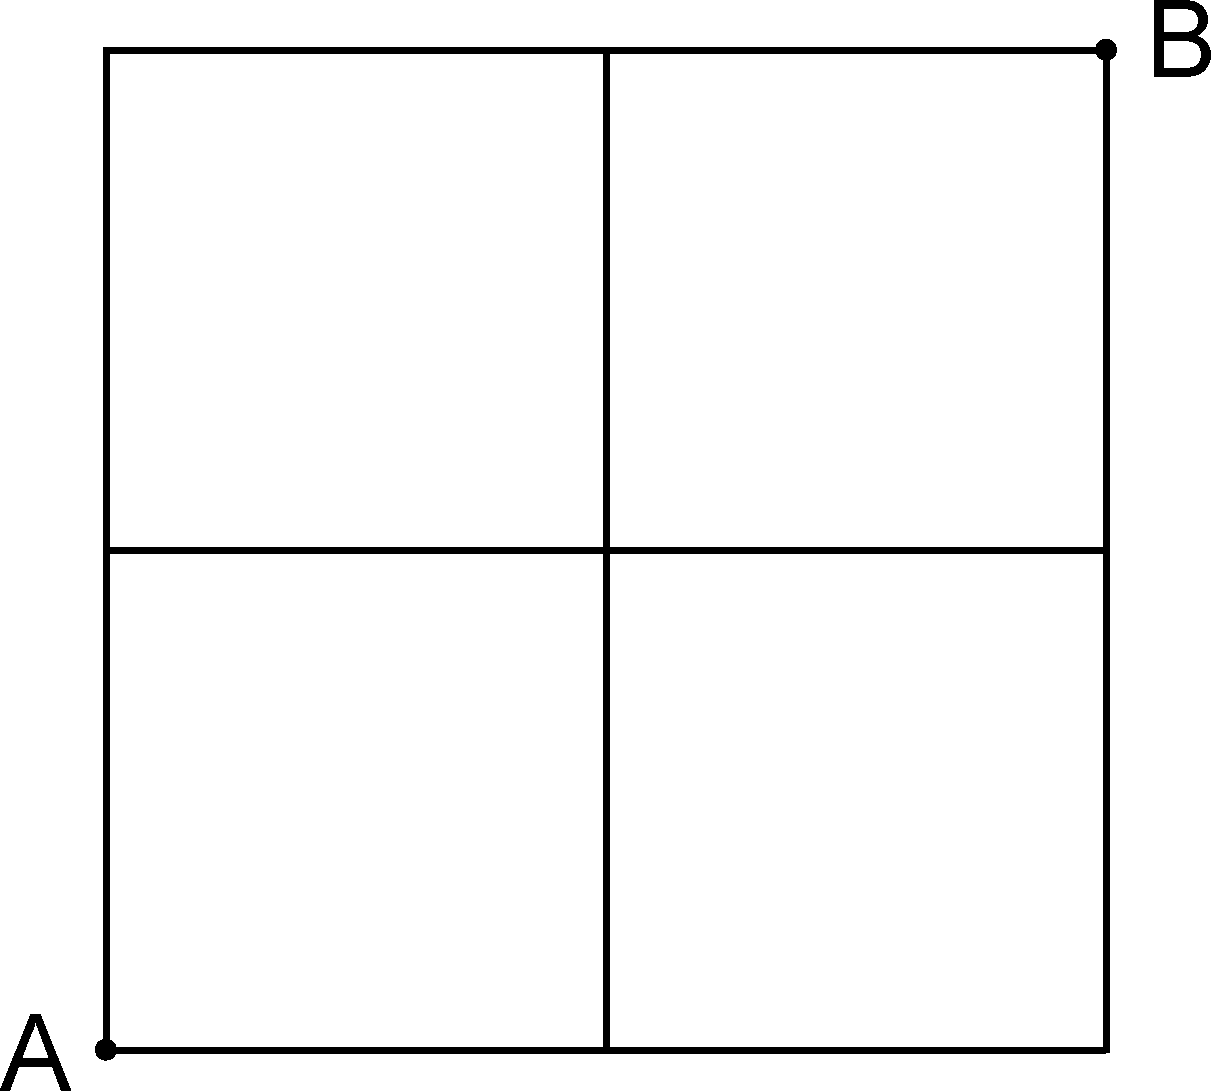
\includegraphics[width=0.2\linewidth]{2014-v3g-01-ruudustik}
\end{center}
\fi


\ifHint
Sümmeetria kaalutlustel saab skeemis sama potentsiaaliga punkte kokku ühendada.
\fi


\ifSolution
Sümmeetria tõttu on ruudustiku kaks tähistamata nurka ja keskpunkt sama potentsiaaliga, mistõttu võid need kolm punkti kokku ühendada. Saadud skeem jaotub ilusti rööp- ja jadaühendusteks, nende abil saame punktide A ja B vaheliseks takistuseks $R=\SI{1,5}{\ohm}$.
\fi


\ifEngStatement
% Problem name: Grid
A 2x2 grid is made out of wire (see figure), the resistance of each small square’s edge is $r=\SI{1}{\ohm}$. Find the resistance between the points A and B. 
\begin{center}
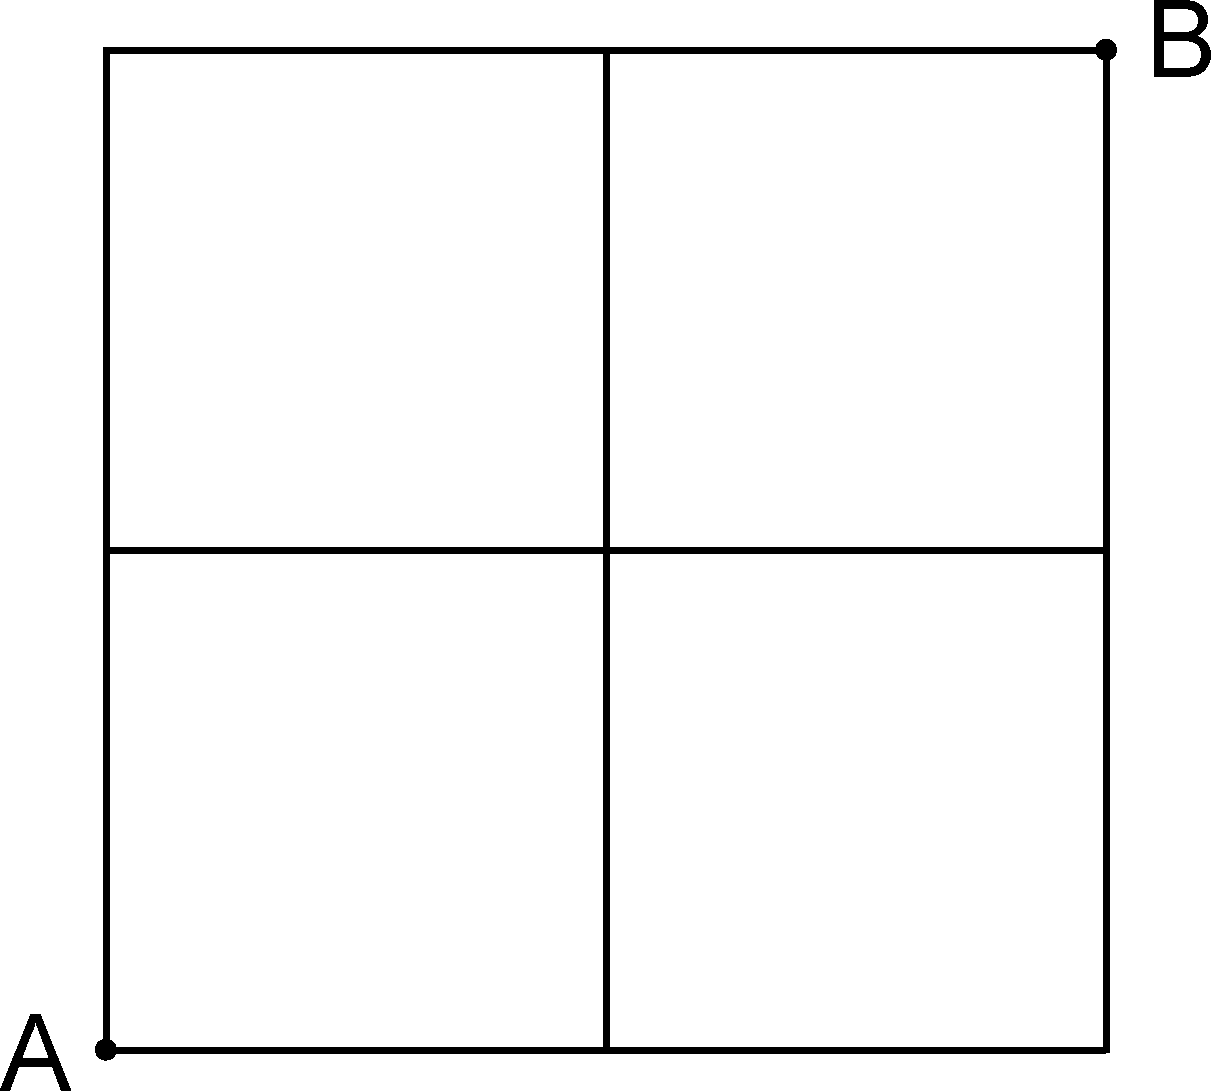
\includegraphics[width=0.2\linewidth]{2014-v3g-01-ruudustik}
\end{center}
\fi


\ifEngHint
Considering the symmetry you can connect the points with the same potential in the scheme.
\fi


\ifEngSolution
Due to symmetry the two unmarked corners and the center of the grid have the same potential, which is why we can connect these three point together. The acquired diagram is nicely divided into parallel and series connections through which we find the resistance between the points A and B to be $R=\SI{1,5}{\ohm}$.
\fi
}